\message{ !name(proposal.tex)}\documentclass[11pt,twocolumn]{article}

\usepackage{amssymb} \usepackage{graphicx} \graphicspath{ {../imgs/} }

\title{Homotopy-aware path planning} \author{Daniel Bencic}
\date{25.08.2022}

\begin{document}

\message{ !name(proposal.tex) !offset(-3) }

\maketitle

\section*{Introduction} One of the crucial tasks for every autonomous
robot is finding a collision free path through free space. Due to it's
importance this problem has been studied for decades and is know as
the path planning or the ``piano movers'' problem
\cite{schwartzPianoMoversProblem1983a,schwartzPianoMoversProblem1983b}. It
has also been shown \cite{reifComplexityMoverProblem1979} that this
problem is PSPACE-complete.

\section*{Problem Formulation}
\subsection*{Preliminaries} This section introduces some fundamental
concepts necessary for describing homotopy-aware path planning
\cite{munkresTopology2014,lavallePlanningAlgorithms2006,hatcherAlgebraicTopology2002}.

\textbf{Homeomorphism} If there exists a bijective function \(f: X
\mapsto Y\) such that \(f\) and it's inverse \(f^{-1}\) are continuous
functions, then the topological spaces \(X\) and \(Y\) are
homeomorphic. Homeomorphism implies that both \(X\) and \(Y\) share
the same topological properties.

\textbf{Configuration Space} Given a metric space \(\mathcal{W}\) with
metric \(d\) and a rigid body \(\mathcal{A}\), a rigid body
transformation is a function \(f: \mathcal{A} \mapsto \mathcal{W}\)
such that \(d(a_{1}, a_{2}) = d(f(a_{1}), f(a_{2}))\) and no
reflection occurs. This holds for rotations and translations. Given
\(GL(n)\) by the set of all invertible \(n \times n\) matrices,
\(O(n)\) is a subgroup of \(GL(n)\) such that \(QQ^{T} = Q^{T}Q = I\)
for all \(Q \in O(n)\). The subgroup \(SO(n)\) of \(O(n)\) which
contains all rotations matrices meaning \(det(P) = 1\) for all \(P \in
SE(n)\). Combining arbitrary rotations and translations gives the
special euclidean group \(SE(n)\) which is homeomorphic to
\(\mathbb{R}^{n} \times SO(n)\).

The configuration space for a rigid robot is therefore \(\mathcal{C}
\cong \mathbb{R}^{2} \times \mathbb{S}^{1}\) and \(\mathcal{C} \cong
\mathbb{R}^{3} \times \mathbb{RP}^{3}\) in 2D space and 3D space,
respectively.

\textbf{Path} Given two point \(x, y \in X\), a path is a continous
function \(f: [0, 1] \mapsto X\) such that \(f(0) = x\) and \(f(1) =
y\). Paths for which \(f(0) = f(1) = x\) are loops with basepoint
\(x\).

\textbf{Homotopy} Two paths \(f\) and \(g\) with the same endpoints
are homotopic if one can be continuously deformed into the
other. Formally, there exists a familiy \(f_{t}: [0, 1] \mapsto X, 0
\le t \le 1\) such that \(f_{t}(0) = x\), \(f_{t}(1) = y\) and
\(f_{0}(s) = f(s)\), \(f_{1}(s) = g(s)\) and the function \(F(s, t):
[0, 1] \times [0, 1] \mapsto X\) defined by \(F(s, t) = f_{t}(s)\) is
continuous (Figure \ref{fig:homotopy}).

\begin{figure}[h] \centering 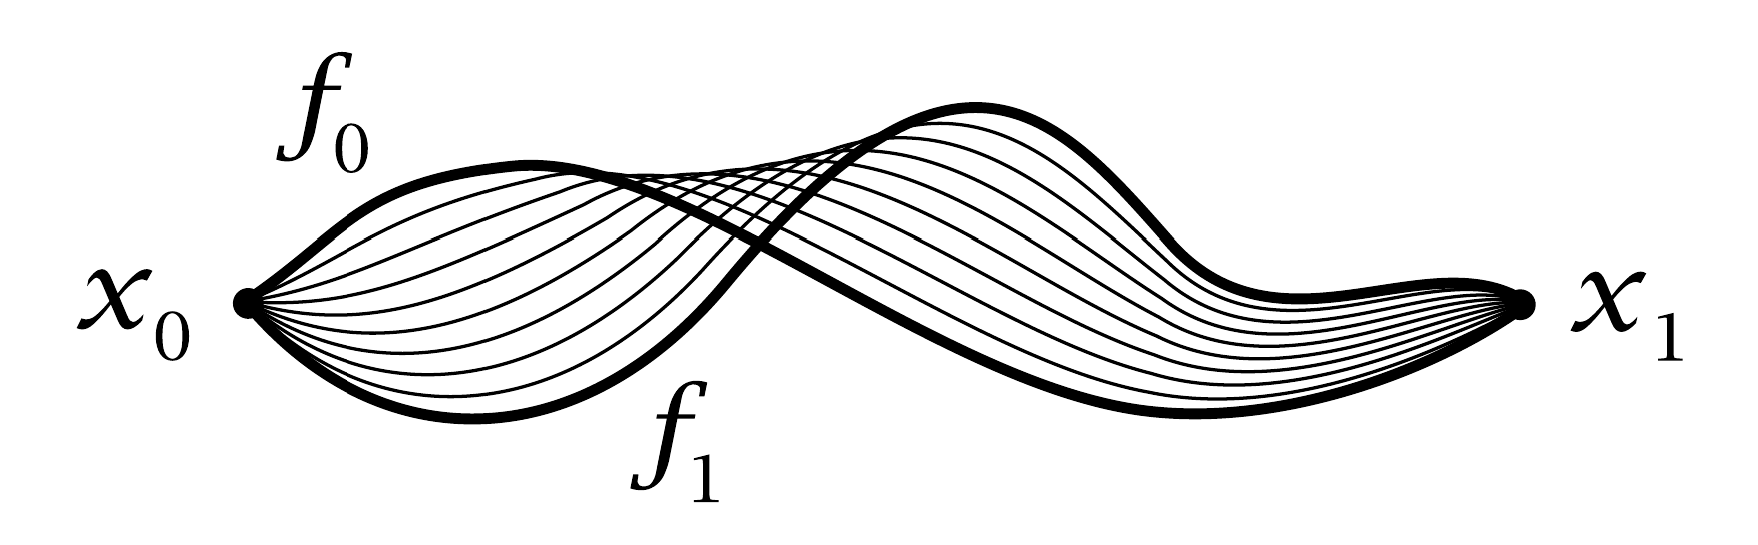
\includegraphics[scale=.18]{homotopy}
  \caption{Homotopy \cite{hatcherAlgebraicTopology2002}.}
  \label{fig:homotopy}
\end{figure}

\subsection*{The Path Planning Problem} Given the set of all possible
transformations of a rigid robot \(\mathcal{C}\) and the
transformations that lead to a collision with obstacles
\(\mathcal{C}_{obs}\), the free space is \(\mathcal{C}_{free} =
\mathcal{C} \setminus \mathcal{C}_{obs}\) (Figure
\ref{fig:cspace}). Let \(q_I\) be the initial configuration and
\(q_G\) the goal configuration. The solution to the path planning
problem is a continuous path \(\pi: [0, 1] \mapsto
\mathcal{C}_{free}\) where \(\pi(0) = q_I\) and \(\pi(1) = q_G\).

\subsection*{Homotopic Path Planning} Homotopic path planning extends
the path planning problem to finding paths for every homotopy
class. Again given \(q_{I}\) and \(q_{G}\), we want to find paths for
different homtopy classes \([f_{n}]\) (see Figure ).

\begin{figure}[h] \centering
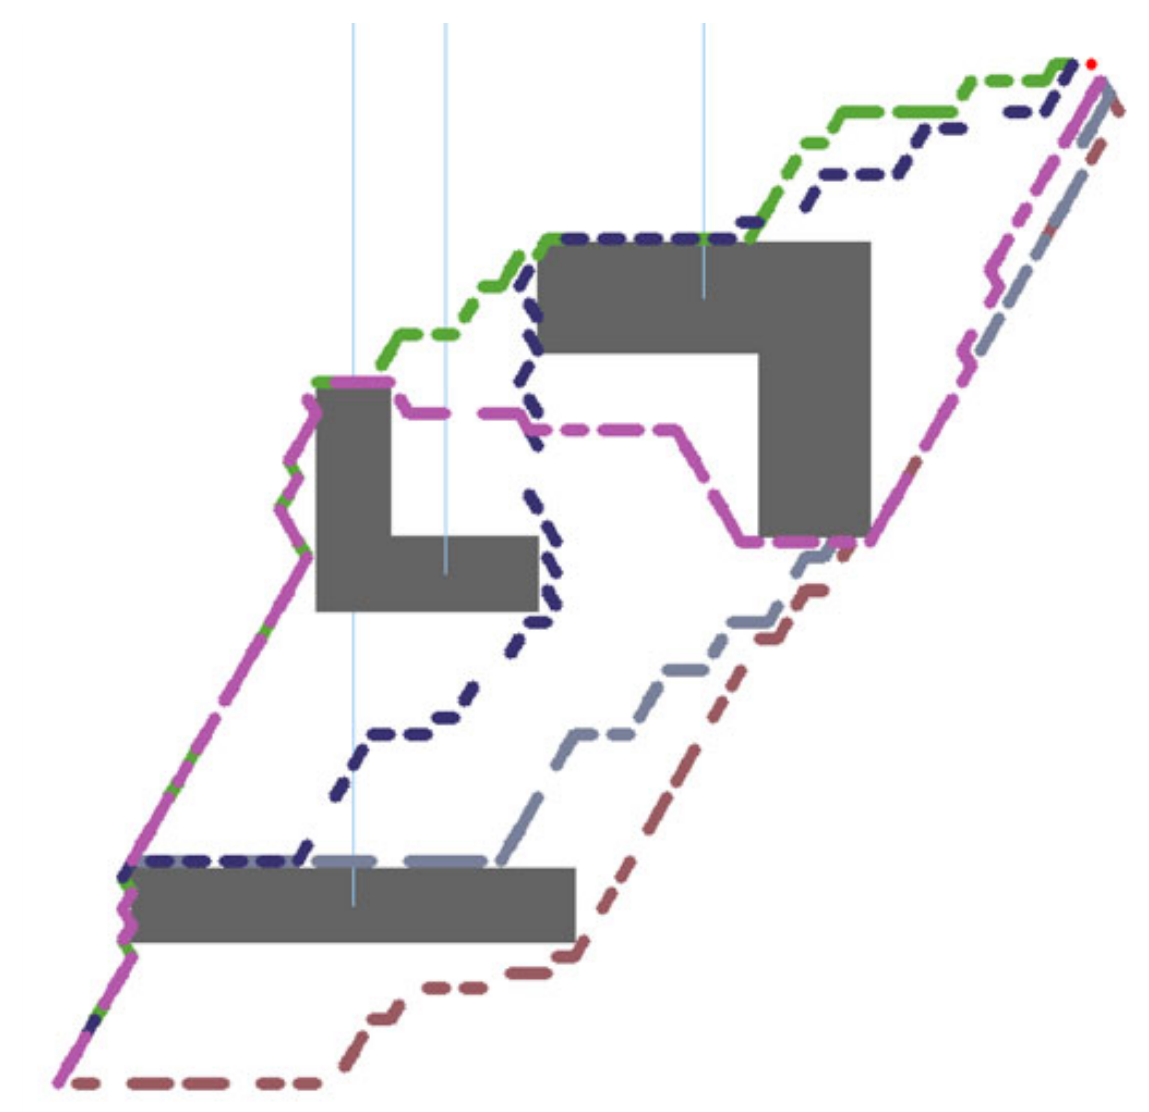
\includegraphics[scale=.2]{homotopy_classes}
  \label{fig:homotopy-classes}
  \caption{Paths belonging to different homotopy classes
\cite{bhattacharyaPathHomotopyInvariants2018}.}
\end{figure}

\begin{figure}[h] \centering 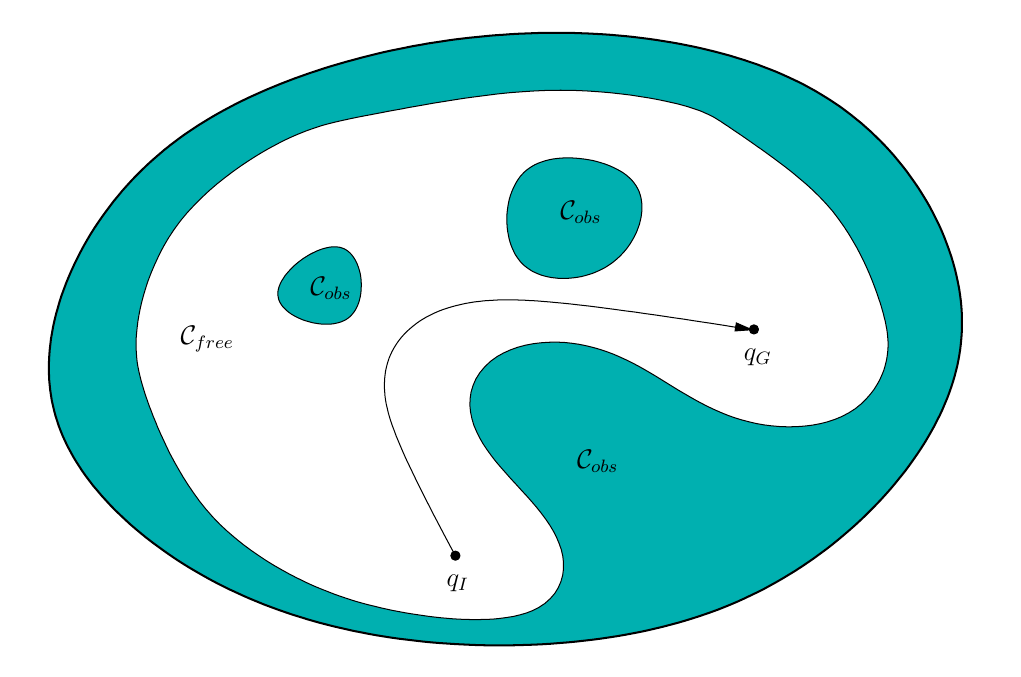
\includegraphics[scale=.25]{cspace}
  \caption{The path planning problem
\cite{lavallePlanningAlgorithms2006}.}
  \label{fig:cspace}
\end{figure}

\section*{Related Work}
\subsection*{Path Planning} Due to the computational complexity of the
path planning problem, there are different approaches to solve this
problem in polynomial time.

\textbf{Graph search}. These approaches assume that \(\mathcal{C}\) is
in the form of a graph. They then apply graph search techniques to
find the path \(\pi\). A widely used algorithm to compute shortest
paths in a graph is Dijkstra's algorithm
\cite{dijkstraNoteTwoProblems1959}. It is a greedy algorithm that
computes the shortest path from every node to every other node in the
graph. The next node for expansion is selected based on the lowest
cost-to-come \(\hat g(x)\). It is \textit{complete}, meaning it finds
a solution if one exists and reports failure otherwise. It is also
\textit{optimal} in the sense that the computed path is the shortest
possible path.

A* \cite{hartFormalBasisHeuristic1968} improves Dijkstra's algorithm
by reducing the number of expanded nodes in the graph. This is
achieved by using a different function \(\hat f(x) = \hat g(x) + \hat
h(x)\) to select the next node for expansion. The term \(\hat h(x)\)
is a heuristic for the least possible cost-to-go in a metric
space. Many path planning algorithms in the current literature build
upon A* (Figure \ref{fig:graph-search}).

\begin{figure}[h] \centering
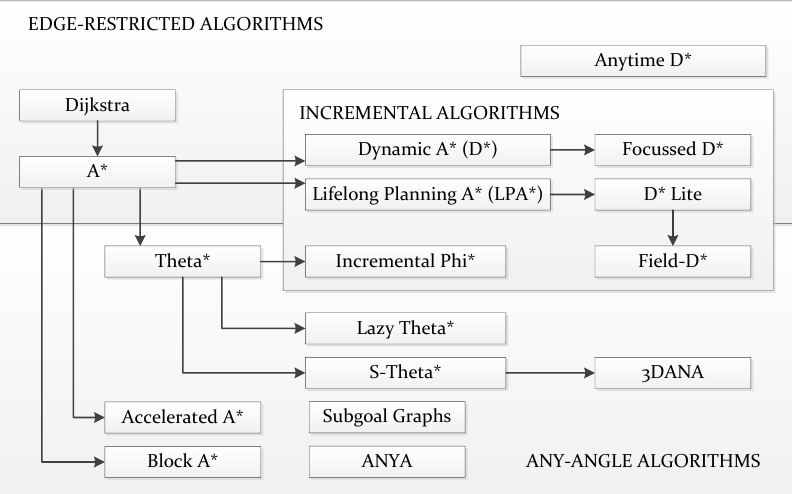
\includegraphics[scale=.35]{graph_search_algorithms}
  \caption{Evolution of graph search algorithms for the path planning
problem \cite{sanchez-ibanezPathPlanningAutonomous2021}.}
  \label{fig:graph-search}
\end{figure}

Stentz et al. developed D*, an incremental algorithm based on A* that
is able to find shortest paths on maps with changing costs, i.e. due
to a robot moving trough the environment and updating the map. D*
computes a path backwards from the goal to the robot. Koenig et
al. \cite{koenigIncremental2001} also proposed an incremental version
of A* (LPA*), where successive runs only recalculate locally
inconsistent nodes. They combined it with the backward search of D*
and created D*-Lite \cite{koenigLite2002}, a less complex version of
D* with at least the same performance therefore making D* obsolete.

Daniel et al. \cite{danielThetaAnyAnglePath2010} showed an approach
specifically for grid-maps that is not limited to predefined angles
for the transition to other grid cells. It is based on A* and uses
line of sight to determine successor nodes. Another any-angle approach
proposed by Ferguson et al.  \cite{fergusonFieldAlgorithmImproved2005}
uses linear interpolation to find the least cost path trough a cell
and produces globally smooth paths.

A comprehensive review of graph search algorithms for the path
planning problem can be found in the literature
\cite{aitsaadiUAVPathPlanning2022,sanchez-ibanezPathPlanningAutonomous2021,yanComprehensiveSurveyAnalysis2020,nashAnyAnglePathPlanning2013}.

\textbf{Sampling}. Due to the curse of dimensionality
\cite{bellmanDynamicProgramming1984}, graph search in high dimensional
configuration spaces can quickly become computationally intractable.
Sampling-based approaches discretize the high-dimensional
configuration space by generating random samples in
\(\mathcal{C}_{free}\). One highly influential contribution from
Kavraki et. al. \cite{kavrakiProbabilisticRoadmapsPath1996} is called
Probabilistic Roadmap Method (PRM). It is a solution to the
multi-query path planning problem in high dimensional configuration
spaces. The method consists of a learning and a query phase. The
former repeatedly generates a random configuration in
\(\mathcal{C}_{free}\) and connects this sample to neighboring nodes
in a given radius with a fast local planner. In addition, a heuristic
is used to generate extra nodes in ``difficult'' regions of
\(\mathcal{C}_{free}\). The method is therefore influenced by the
topological properties of \(\mathcal{C}_{free}\). The result is a
graph representation of \(\mathcal{C}_{free}\) in the form of a forest
of trees.

Another highly cited approach using only a single tree is the
Rapidly-exploring Random Tree (RRT) algorithm by Lavalle
\cite{lavalleRapidlyExploringRandomTrees1998}. The algorithm grows a
tree in \(\mathcal{C}_{free}\) by generating a sample from a uniform
distribution and growing the nearest node of the tree in the direction
of the sample. Since the probability that a node is selected for
expansion is proportional to the size of it's Voronoi cell (see Figure
\ref{fig:rrt}), the tree grows with a bias towards unexplored regions
in \(\mathcal{C}_{free}\).

Karaman et. al. \cite{karamanSamplingbasedAlgorithmsOptimal2011}
showed that both PRM and RRT algorithms are not asymptotically
optimal. That means that with a growing number of nodes the
probability that the algorithm finds an optimal solution converges to
zero. In their paper they also proposed two new algorithms PRM* and
RRT* which are shown to be asymptotically optimal. The former was
improved by calculating the radius, in which a sample is connected to
it's neighbors, based on the number of present samples. The latter was
improved by selecting the node for expansion based on the cost-to-come
in the neighborhood of a sample and rewiring the tree after insertion
of a new node.

There are many algorithms improving and extending RRT and RRT* in the
literature. With RRT-Connect, Kuffner et. al.
\cite{kuffnerRRTConnectEfficientApproach} introduced a bidirectional
RRT that grows one tree from \(q_I\) and another tree from \(q_G\)
while trying to connect the two trees. Anytime RRT*
\cite{karamanAnytimeMotionPlanning2011} returns a fast initial
solution and a robot commits to execute a subset of the full path
\(\pi_{com}: [0, t_{com}] \mapsto C_{free}\). While executing
\(\pi_{com}\) the remaining path is further improved until the robot
commits to the next subset of the path. Realizing that there is a
subset of \(C_{free}\) that contains configurations that are
guaranteed to improve the current solution, Informed RRT*
\cite{gammellInformedRRTOptimal2014} uses a ellipsoidal heuristic to
sample from this set and improve the convergence rate of RRT*. BIT*
\cite{gammellBatchInformedTrees2015} does not sample a single
configuration, instead it samples a batch of configurations and grows
a tree from this batch.  After finding a solution or no further
possible expansion, the next batch is sampled. If a solution has been
found with the previous batch, this batch is sampled from the
ellipsoidal subset introduced by Informed RRT* and the tree is updated
by identifying locally inconsistent nodes.

A comprehensive review of RRT* variants has been published by Noreen
et. al.  \cite{noreenOptimalPathPlanning2016a} and a review of more
sampling-based approaches for the path planning problem can be found
in \cite{elbanhawiSamplingBasedRobotMotion2014}.

\subsection*{Homotopy-awareness} Most algorithms for solving the path
planning problem focus on finding one path which is optimal in terms
of a specific metric. The majority of these algorithms is of course
influenced by the topological properties of the configuration space,
but they do not explicitly model them. However these properties are
crucial for the semantic understanding of the configuration space.

Bhattachary et. al. \cite{bhattacharyaPathHomotopyInvariants2018}
constructed homotopy invariants for a \(D\)-dimensional manifold \(X\) by
introducing \((D - 1)\)-submanifolds. They then construct words by
tracing a path \(f\) and inserting a letter every time \(f\) intersects
one of the submanifolds. They then construct a \(h\)-augmented graph.
Given a graph \(G = (V, E)\), the \(h\)-augmented graph is a lift
of \(G\) into the covering space of \(X\). They then are able to use
traditional graph search algorithms to find paths in different homotopy
classes.

\begin{figure}[h] \centering 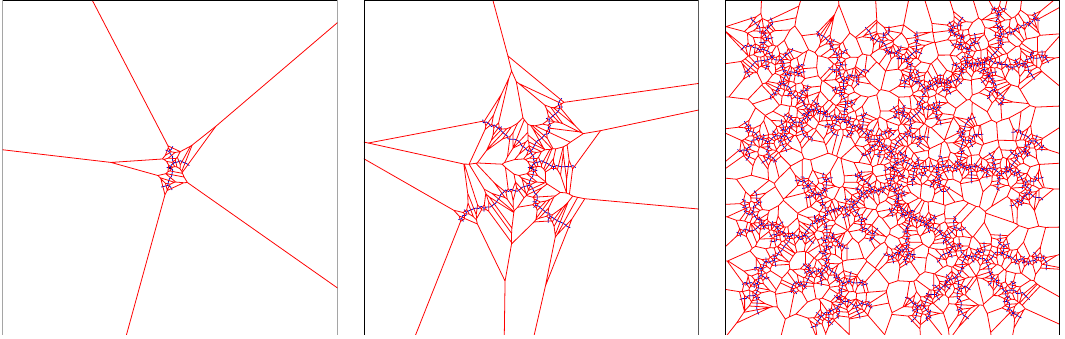
\includegraphics[scale=.275]{rrt_voronoi}
  \caption{Voronoi diagram of a RRT tree.}
  \label{fig:rrt}
\end{figure}

\bibliographystyle{plain} \bibliography{../bib/mybib}

\end{document}

\message{ !name(proposal.tex) !offset(-245) }
